\documentclass{csse4400}

% \teachermodetrue

\usepackage{float}

\usepackage{languages}

\title{Storing Stuff // TODO}
\author{Evan Hughes \& Brae Webb}

\date{\week{3}}
\begin{document}

\maketitle

\begin{figure}[h]
  \href{https://www.oreilly.com/library/view/designing-data-intensive-applications/9781491903063/ch02.html}{
    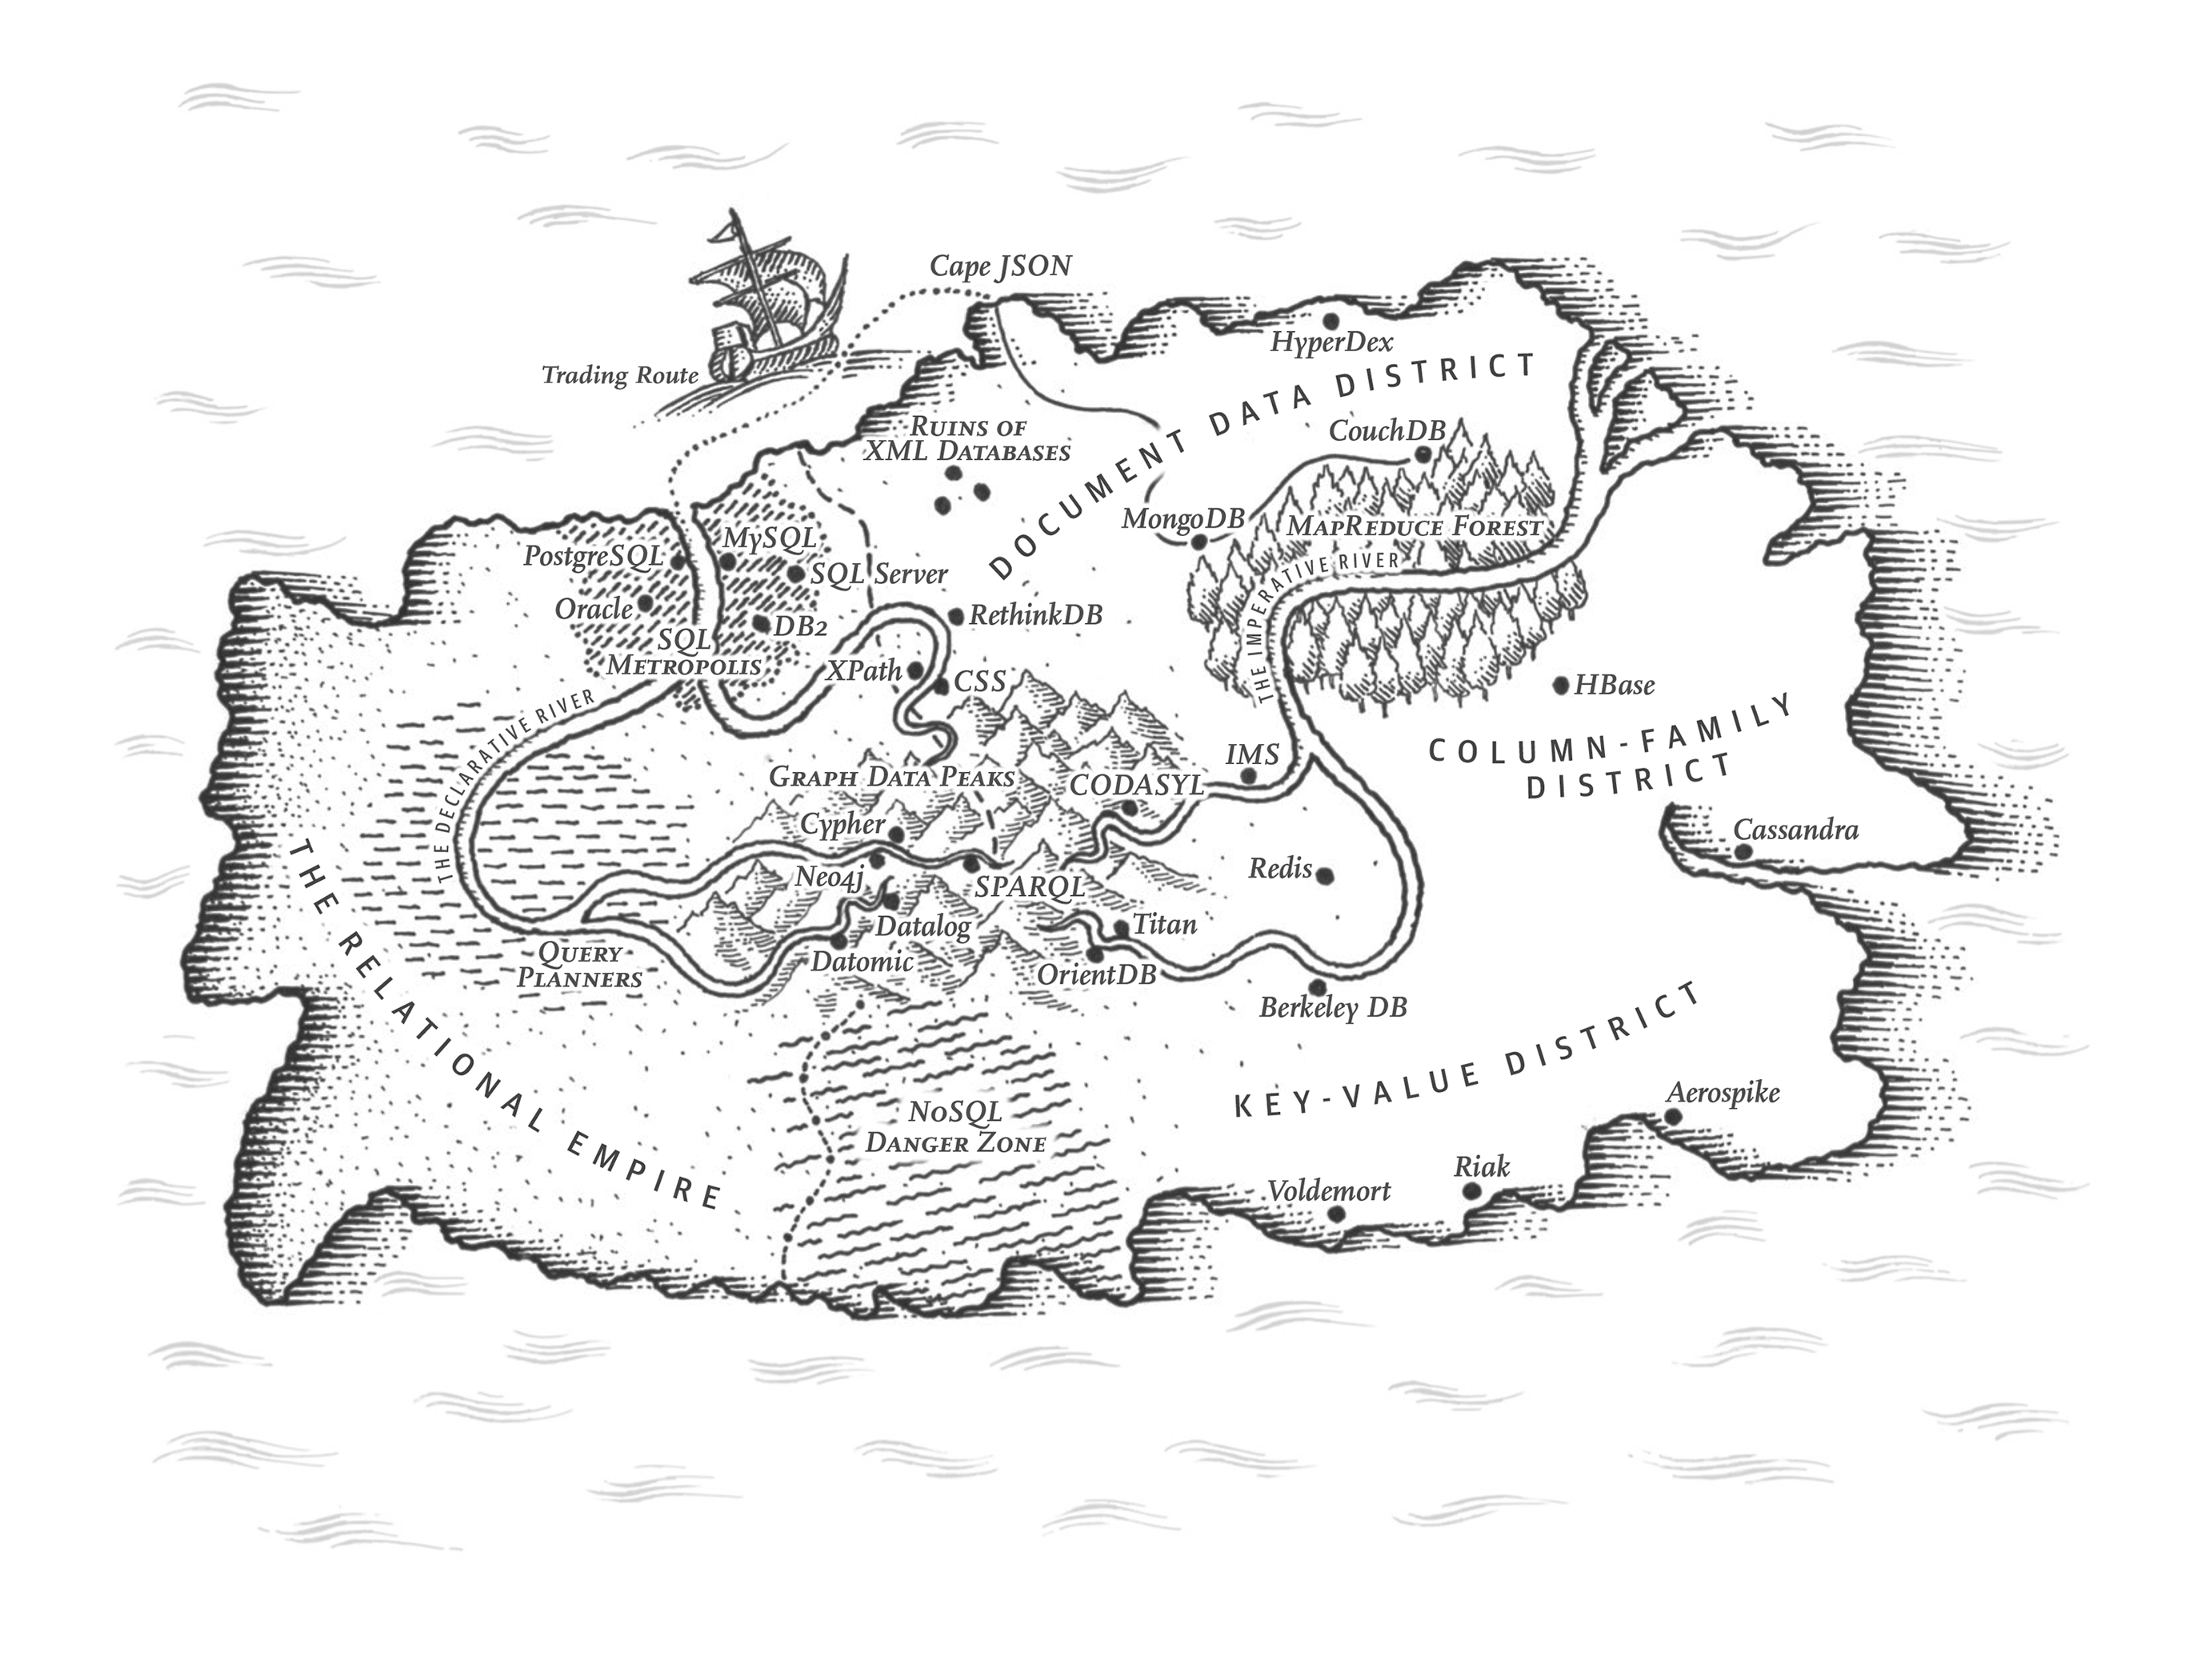
\includegraphics[width=\textwidth]{images/databases}
  }
\caption{A map of data storage techniques from Designing Data-Intensive Applications \cite{data-intensive}.}
\end{figure}

\section{This Week}
This week our goal is to:
\begin{itemize}
  \item explore the various techniques developers use to store data;
  \item investigate the storage options implementing these techniques on the AWS platform;
  \item run a small application using docker that requires a database; and
  \item deploy the application in AWS using Terraform.
\end{itemize}

\section{Databases and Data Models}
Unfortunately, to build interesting software we often need to store and use data.
The storage of data introduces a number of challenges when designing, creating, and maintaining our software.
However, not all data storage techniques are created equal;
the choice of data storage model can have a profound impact on our software's complexity and maintainability.
In this practical, we want to take a superficial exploration of our island of data storage models.
For a more in-depth treatment of data storage models that is outside the scope of this course,
see Chapter 2 of the \textit{Designing Data-Intensive Applications} book \cite{data-intensive}.

\teacher{
  Discuss the following different storage technologies and mention some use cases of when you would choose each one.
  Discuss some popular implementations of each.\\

  Aim for no more than 30 minutes of discussion.
}

\subsection{Relational Storage}

Relational databases what have been exposed to the most in your University career --- think MySQL, Postgres, Oracle DB, etc.
This type of database is good at modelling the real world which is often a highly connected environment.
% The data model that is suggested for this type of storage is a normalised approach where data duplication should be reduced.

Some popular offerings are below:

\begin{itemize}
  \item MySQL/MariaDB [ Amazon RDS / Amazon Aurora ].
  \item Postgres [ Amazon RDS / Amazon Aurora ].
\end{itemize}

The AWS offerings of these services come in two different types, we have the traditional approach of
server capacity ( x cores, y ram ) and we have a server-less approach.
The server-less approach is a more dynamic
database that can scale to large amounts of load when needed though at a cost per request.

  \subsubsection{ORM}
  Object Relational Mapping (ORM) is a fairly common tool for programmers to use to make developing with databases smoother.
  One fairly prevalent example of this is SQLAlchemy which is a very widely used 
  database abstraction for python.
  SQLAlchemy allows us to move to a higher level of abstraction than SQL queries and perform database actions using standard python code.

  The benefits of ORMs are the ability to model database objects in our existing programming language instead of having large blocks of SQL text within our source code.
  The disadvantages come in when we need to do specific SQL work or where the abstractions cost is greater than the benefits.

\subsection{Wide-Column Storage}

\teacher{
  Examples of big apps that depend on this technology is Netflix \url{https://netflixtechblog.com/netflixs-viewing-data-how-we-know-where-you-are-in-house-of-cards-608dd61077da}.
}

Wide-Column databases are a form of NoSQL or non-relational data stores.
In these data stores the data model design 
is focused more on having efficient queries at the cost of data duplication.
A warning to the reader that these models
are not flexible after creation, it is much easier to answer a new use case in a relational model.

  \begin{itemize}
    \item Apache Cassandra [ Amazon Keyspaces for Cassandra ].
    \item Apache HBase.
  \end{itemize}

\subsection{Key-Value Storage}

Key-Value stores are very popular for cache or remote config use cases, some of the most notable are Redis and Memcached.
These stores allow efficient lookup of values via keys and are usually stored in-memory.

\begin{itemize}
  \item Redis [ Amazon ElastiCache for Redis ].
  \item Memcached [ Amazon ElastiCache for Memcached].
  \item Amazon DynamoDB.
  \item Amazon MemoryDB for Redis.
\end{itemize}

\subsection{Time Series Storage}

\teacher{
  Something to mention here is that relations are usually not utilised between tables in time series databases.
}

Time series databases are highly focused storage which is tailored to retrieving results by timestamp ranges.
Many implementations also take advantage of the data model to allow efficient rollover of data and partitioning.
One of the most popular time series databases is Prometheus which is used to store monitoring metrics.

\begin{itemize}
  \item Amazon Timestream.
  \item TimescaleDB ( Postgres + Addon ).
  \item Prometheus.
  \item InfluxDB.
\end{itemize}

\subsection{Document Storage}

Document databases are a subset of NoSQL databases with a focus on a flexible data model.
MongoDB for instance allows the user to store JSON documents and perform queries on those documents.
One advantage of document databases is that they match a programmers existing mental model of storing data in formats such as JSON.

\begin{itemize}
  \item MongoDB.
  \item Apache CouchDB.
  \item Amazon DocumentDB.
  \item Amazon DynamoDB.
\end{itemize}

\subsection{Graph Storage}

\teacher{
  If you havnt experienced graph databases, a good usecase is ``recommendation systems'',
  which use the connected nature of items to figure out what to suggest to a person.Another example is the \url{https://neo4j.com/blog/analyzing-panama-papers-neo4j/}
  Panama Papers.
}

Graph Databases are relational storage with a few enhancements to allow fast neighbour look-ups.
These databases also allow the implementation of graph algorithms to query data.

\begin{itemize}
  \item Amazon Neptune.
  \item Neo4J.
  \item Janus Graph.
\end{itemize}

\section{Deploying an Application with Storage}

Thus far in the course we have introduced docker in small packages which do not communicate (much) with the outside world.
Today we will be using it to run an application which needs to talk to a database.
\begin{enumerate}
\item First we will deploy the application and database locally.
\item Then we will deploy the database on AWS infrastructure and configure our application to talk to the remote database.
\item Finally, we will deploy the application and database on AWS infrastructure.
\end{enumerate}

\begin{figure}[H]
  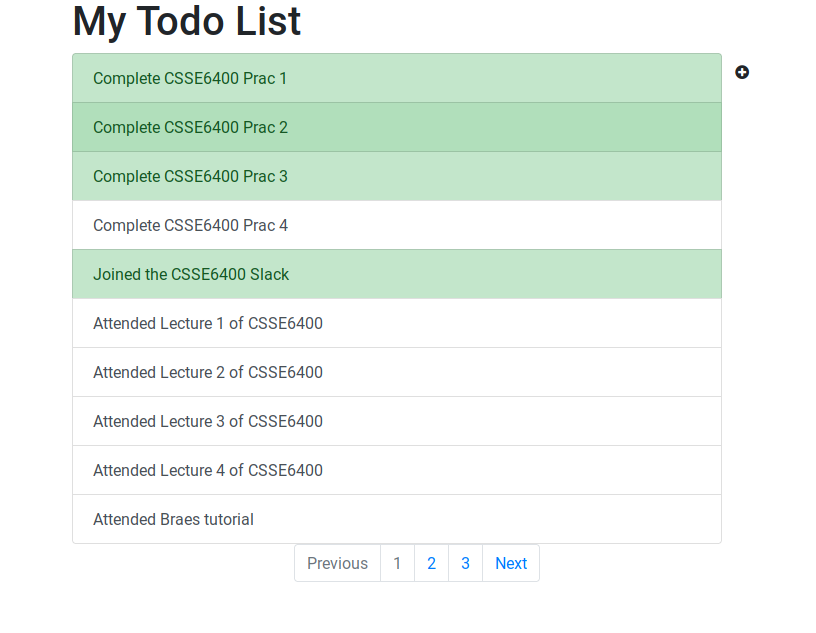
\includegraphics[width=\textwidth]{images/todoapp}
\caption{Sample Todo App made for the course}
\end{figure}

\info{
    You will need to have docker and docker-compose installed for this practical.
    Installation will depend on your operating system.

    \begin{itemize}
      \item Docker compose: https://docs.docker.com/compose/install/
      \item Docker engine: https://docs.docker.com/get-docker/
    \end{itemize}
    
    We also recommend installing the vscode docker plugin or the equlivant tools in IntelliJ IDEs.
}

\aside{
  We have only seen individual Docker containers running thus far.
  As we start to build distributed systems,
  we will want to use multiple Docker containers which talk to each other.
  Docker compose is a container orchestration tool that allows us to configure multiple containers to run and setup paths for them to talk to each other.
}

\teacher{
  Wait for students to get docker-compose installed,
  they should have docker from their tutorials but some may be missing it.
}

\warning{
    For terminal examples in this section,
    lines that begin with a \$ indicate a line which you should type while the other lines are example output that you should expect.
    Not all of the output is captured in the examples to save on space.  
}

\section{Deploying Locally}

\teacher{
  Mention that the dockerfile exists but no need to get the repo.
  We will not be building the container ourselves.
  Instead use one that is published on the github,
  shown further down in the docker-compose.
}

We will be using a container that is pre-built from the Dockerfile below.
You should browse the contents of this container to gain more exposure to Dockerfile although you aren't required to use the file for this task --- we will use an image already built from this Dockerfile.

\begin{code}[language=docker]{Dockerfile}
FROM ubuntu:21.10
RUN apt-get update \
        && DEBIAN_FRONTEND=noninteractive apt install -y \
            php \
            php-mysql \
            php-xml \
            php-curl \
            curl \
            git \
            unzip
RUN curl -sS https://getcomposer.org/installer | php -- --install-dir=/usr/local/bin --filename=composer
COPY . /app
WORKDIR /app
RUN composer install
CMD ["php", "artisan", "serve", "--host=0.0.0.0"]
\end{code}

Our first task is to have a local instance of the Todo App including the database.
To get started we need to make a new directory for our work and create a Docker compose file.

\begin{code}[language=shell,numbers=none]{}
  $ mkdir prac4 && cd prac4
  $ touch docker-compose.yml
\end{code}

Docker Compose is a small helper utility that allows us to more easily run docker applications without needing to remember a lot of command line parameters.
Instead we define how we want our docker container to run through a YAML config file.
Insert the following into your docker-compose.yml file.

\begin{code}[language=docker-compose]{docker-compose.yml}
version: '3.3'
services:
  backend:
    image: ghcr.io/csse6400/todo-app:latest
    ports:
      - '8000:8000'
    environment:
      APP_ENV: 'local'
      APP_KEY: 'base64:8PQEPYGlTm1t3aqWmlAw/ZPwCiIFvdXDBjk3mhsom/A='
      APP_DEBUG: 'true'
      LOG_LEVEL: 'debug'
\end{code}

\teacher{
  Feel free to show students dockerhub and where on github this container is stored. URL for 
  this container is here \url{https://github.com/CSSE6400/todo-app/pkgs/container/todo-app}
}

A few things to point out in the file.
We have defined a single service (container) called backend which uses the pre-built docker image from \url{ghcr.io/csse6400/todo-app} with the tag of latest.
We then have exposed this onto our machine on port 8000 and have passed a few environment variables required for the application.%\lstinline{docker-compose up}.

\lstinline{docker-compose up} will use our docker compose configuration to run any containers we have specified.

\begin{code}[language=shell,numbers=none]{}
  $ docker-compose up
  Creating network "p1_default" with the default driver
  Creating p1_backend_1 ... done
  Attaching to p1_backend_1
  backend_1  | Starting Laravel development server: http://0.0.0.0:8000
  backend_1  | [Sun Mar 20 07:56:23 2022] PHP 8.0.8 Development Server (http://0.0.0.0:8000) started
\end{code}

Now we head to our browser and go to \url{http://127.0.0.1:8000},
you should be presented with the following screen.

\begin{figure}[ht]
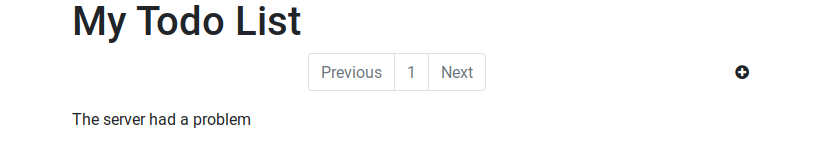
\includegraphics[width=\textwidth]{images/app-missing-db}
\end{figure}

When we see unhelpful error messages such as this,
we should investigate the web console in our browser.
The web console will tell us which network calls are being made and which calls are causing the error message.
Follow along with your tutor to find that the offending network call is to \url{http://127.0.0.1:8000/api/v1/todo}.

Once we open that address we have a clearer idea of what has gone wrong.
The page you should see is shown in Figure \ref{fig:expected-error} and the reason is that our backend cannot connect to a database (because we have yet to make one).

\begin{figure}[H]
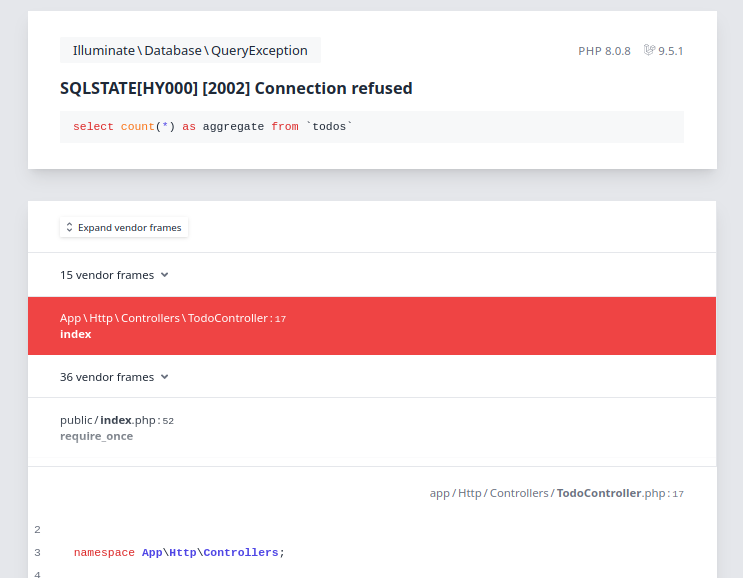
\includegraphics[width=\textwidth]{images/missing-db}
\caption{The expected error page when accessing \url{http://127.0.0.1:8000/api/v1/todo}.}
\label{fig:expected-error}
\end{figure}

To fix this lets add a popular relation database, MySQL, to our docker-compose file.
Edit your docker compose file to match as shown below.

\begin{code}[language=docker-compose]{main.tf}
version: '3.3'
services:
  db:
    image: mysql:8-debian
    environment:
      MYSQL_DATABASE: 'todoapp'
      MYSQL_USER: 'todoapp'
      MYSQL_PASSWORD: 'password'
      MYSQL_ROOT_PASSWORD: 'password'
    ports:
      - '3306:3306'

  backend:
    image: ghcr.io/csse6400/todo-app:latest
    depends_on:
      - db
    ports:
      - '8000:8000'
    environment:
      APP_ENV: 'local'
      APP_KEY: 'base64:8PQEPYGlTm1t3aqWmlAw/ZPwCiIFvdXDBjk3mhsom/A='
      APP_DEBUG: 'true'
      LOG_LEVEL: 'debug'
      DB_CONNECTION: 'mysql'
      DB_HOST: 'db'
      DB_PORT: '3306'
      DB_DATABASE: 'todoapp'
      DB_USERNAME: 'todoapp'
      DB_PASSWORD: 'password'
\end{code}

Now we have two services (containers) for our app and we have added a few more environment variables for our backend to know how to connect to the database.
The \texttt{DB\_HOST} variable uses a feature of docker compose where you can refer to other services by their name rather than a traditional IP address.
This makes it easy for us to setup communication between these two services.

From the same shell let's re-run our containers,
you may need to CTRL+C to stop the current running containers.
Once they have shutdown, run the up command again.

\begin{code}[language=shell,numbers=none]{}
  $ docker-compose up
  Starting p2_db_1 ... done
  Starting p2_backend_1 ... done
  Attaching to p2_db_1, p2_backend_1
  db_1       | 2022-03-20 08:11:55+00:00 [Note] [Entrypoint]: Entrypoint ....
  db_1       | 2022-03-20 08:11:55+00:00 [Note] [Entrypoint]: Switching t....
  db_1       | 2022-03-20 08:11:55+00:00 [Note] [Entrypoint]: Entrypoint ....
  db_1       | 2022-03-20T08:11:55.438996Z 0 [System] [MY-010116] [Server....
  db_1       | 2022-03-20T08:11:55.445261Z 1 [System] [MY-013576] [InnoDB....
  backend_1  | Starting Laravel development server: http://0.0.0.0:8000
  db_1       | 2022-03-20T08:11:55.535803Z 1 [System] [MY-013577] [InnoDB....
  db_1       | 2022-03-20T08:11:55.673757Z 0 [Warning] [MY-010068] [Serve....
  db_1       | 2022-03-20T08:11:55.673784Z 0 [System] [MY-013602] [Server....
  db_1       | 2022-03-20T08:11:55.674810Z 0 [Warning] [MY-011810] [Serve....
  db_1       | 2022-03-20T08:11:55.684729Z 0 [System] [MY-010931] [Server....
  db_1       | 2022-03-20T08:11:55.684756Z 0 [System] [MY-011323] [Server....
  backend_1  | [Sun Mar 20 08:11:55 2022] PHP 8.0.8 Development Serv....
\end{code}

Now when we go to \url{http://127.0.0.1:8000/api/v1/todo} we see a different error message, as shown in Figure \ref{fig:missing-tables}.
This error is complaining that we have a database that we can connect to but the todos table doesn't exist.

\begin{figure}[ht]
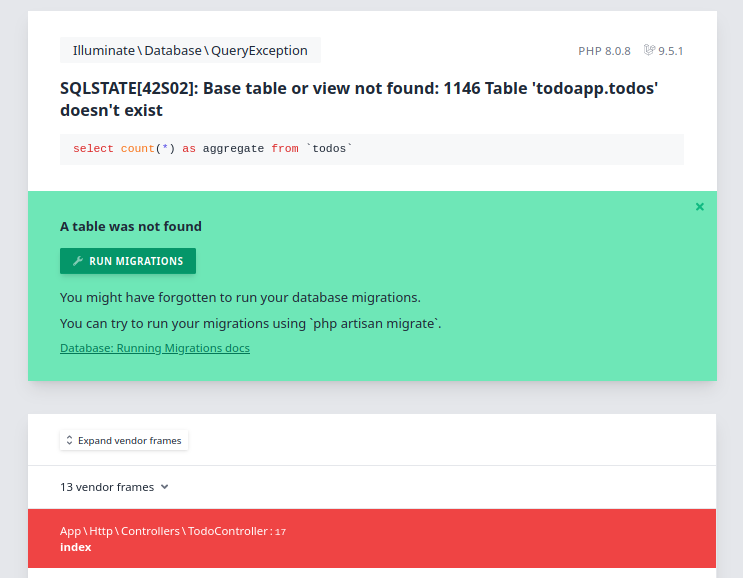
\includegraphics[width=\textwidth]{images/missing-tables}
\caption{The expected error page when accessing \url{http://127.0.0.1:8000/api/v1/todo} after creating a database.}
\label{fig:missing-tables}
\end{figure}

To populate the database our application comes with database migration files.
One way would be to click the ``RUN MIGRATIONS'' button shown on the error page but we also want to pre-populate our database with some dummy data as well.

To do this we are going to jump into the running container and execute the migrations ourselves, using \texttt{docker-compose exec}.
Start by opening a new terminal so that we can leave the docker containers running.
In this new terminal navigate to \textbf{the directory where \texttt{docker-compose.yml} lives} and run the following 
command:

\begin{code}[language=shell,numbers=none]{}
$ docker-compose exec backend php artisan migrate:fresh --seed
Dropped all tables successfully.
Migration table created successfully.
Migrating: 2022_03_19_041557_create_todos_table
Migrated:  2022_03_19_041557_create_todos_table (7.55ms)
Seeding: Database\Seeders\TodoSeeder
Seeded:  Database\Seeders\TodoSeeder (6.56ms)
Database seeding completed successfully.
\end{code}

\noindent Now with this run we can check back at our web app (at \url{http:127.0.0.1:8000})and you should see a fully functional todo app.

\begin{figure}[ht]
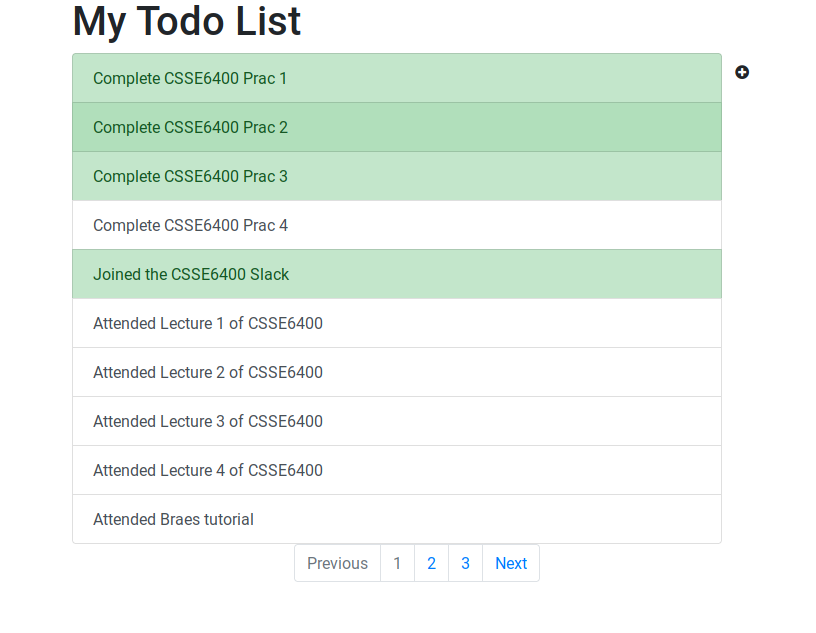
\includegraphics[width=\textwidth]{images/todoapp}
\end{figure}

\info{
  The database migrations are performed by Laravel which is a popular PHP web framework.
  In the database it has created a table to keep track of which migrations have already been run so that it will skip them latter.
  To enable this functionality you will have to edit migrate:fresh to just migrate.\\

  For a production instance you would also typically remove the --seed parameter as you do not want to insert dummy data into your production database.
}

\subsection{Exercise: Migrations at startup}

So far when we run this application we have to perform the database migrations manually. 
To help us get up and running we are going to make a small modification to pre-run the migrations when are web app starts.
First we need to have a look at how the container is set to launch by default.
In the Dockerfile attached at the start of the practical we see that we have defined the command to run on the last line with the CMD directive.

\begin{code}[language=docker]{Dockerfile}
  FROM ubuntu:21.10
  ... 
  ... 
  ...
  CMD ["php", "artisan", "serve", "--host=0.0.0.0"]
\end{code}

\info{
  When working with docker it can get confusing around the networking aspects. In this application I have specified
  that the server must listen on all network interfaces ( 0.0.0.0 ). Without this flag the default is 127.0.0.1 which
  even though its the localhost the forwarded traffic through the docker container would never reach it.
}

This command launches the laravel development server and listens on all interfaces on the host.
We are going to override this in our docker-compose file so that we run the migrations then start the server.
Add the following line to the docker-compose.yml that you have been developing during the practical.

\begin{code}[language=docker-compose]{}
  command: sh -c "sleep 30 && php artisan migrate:refresh --seed && php artisan serve --host=0.0.0.0"
\end{code}

This new command does the following:

\begin{itemize}
  \item Waits for the database to be ready in a simple way.
  \item Runs the migrations and seeds the database, as we have seen earlier.
  \item Starts the development server as the container originally did.
\end{itemize}

Example: condensed version of the goal \texttt{docker-compose.yml} attached below.

\begin{code}[language=docker-compose]{docker-compose.yml}
  version: '3.3'
  services:
    db:
      ...
  
    backend:
      ...
      environment:
        ...
      command: sh -c "sleep 10 && php artisan migrate:refresh --seed && php artisan serve --host=0.0.0.0"
\end{code}

Now when we launch the docker-compose we can see that our migrations were run in the output.

\begin{code}[language=shell,numbers=none]{}
  $ docker-compose up
  ...
  ...
  backend_1  | Rolling back: 2022_03_19_041557_create_todos_table
  backend_1  | Rolled back:  2022_03_19_041557_create_todos_table (8.28ms)
  backend_1  | Migrating: 2022_03_19_041557_create_todos_table
  backend_1  | Migrated:  2022_03_19_041557_create_todos_table (11.55ms)
  backend_1  | Seeding: Database\Seeders\TodoSeeder
  backend_1  | Seeded:  Database\Seeders\TodoSeeder (44.77ms)
  backend_1  | Database seeding completed successfully.
  backend_1  | Starting Laravel development server: http://0.0.0.0:8000
  backend_1  | [Sun Mar 20 12:08:41 2022] PHP 8.0.8 Development Server (http://0.0.0.0:8000) started
\end{code}

We can also bake this into the container by extending the original,
it is fairly common to see projects in the wild that run a init script when the container launches.
An exercise left for the reader is to build upon the provided docker container by including an init script.

\section{Deploying a Database in AWS}

Now we have a locally running Todo App let's move to AWS,
start up your Learner Lab environment now.
This is the last time we will heavily use the AWS user interface in the practicals.
If you already feel confident in the AWS environment skip to Section \ref{sect:terraform} for the terraform setup.

\teacher{
  Give students time to start the labs, could take up to 10 minutes.
}

To get started let's jump into the lab environment and have a look at AWS RDS which is an AWS managed database service.
To get to the RDS service either search it or browse Services -> Database -> RDS as shown below.

\begin{figure}[H]
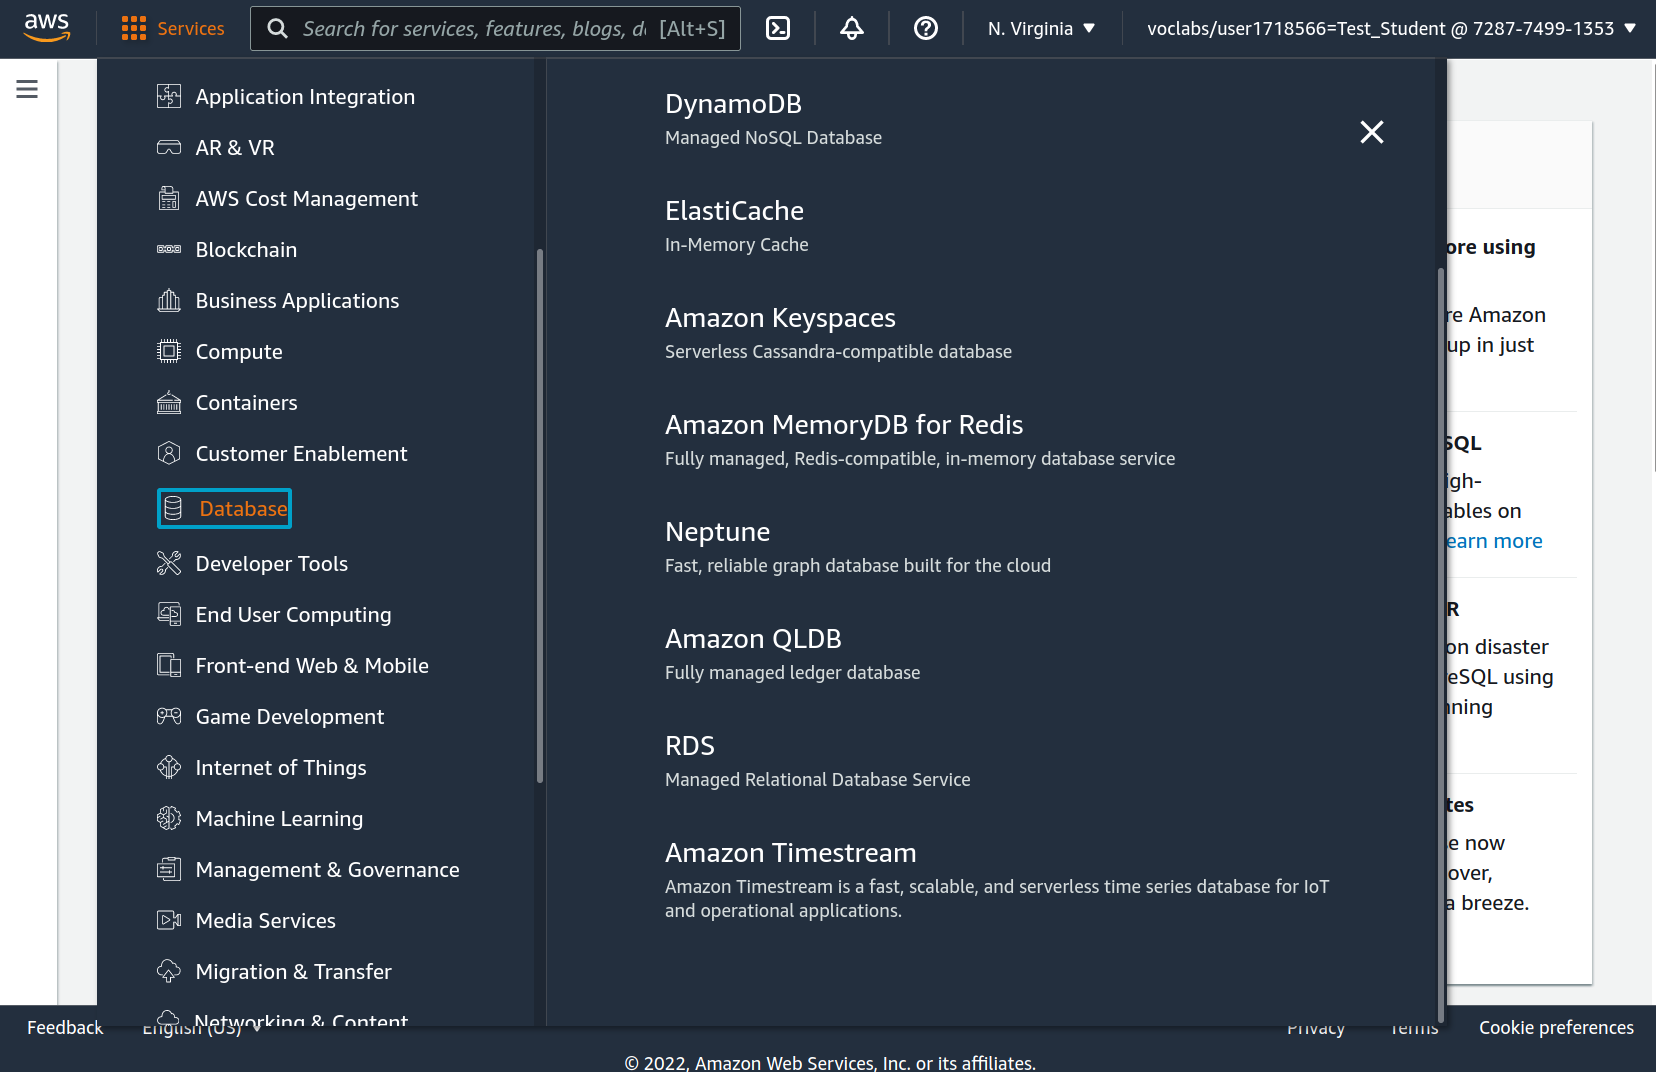
\includegraphics[width=\textwidth]{images/aws_1}
\end{figure}

Now we are in the management page for all our database instances,
for today we just want to get a small instance running to explore the service.
Head to ``DB Instances (0/40)''.

\begin{figure}[H]
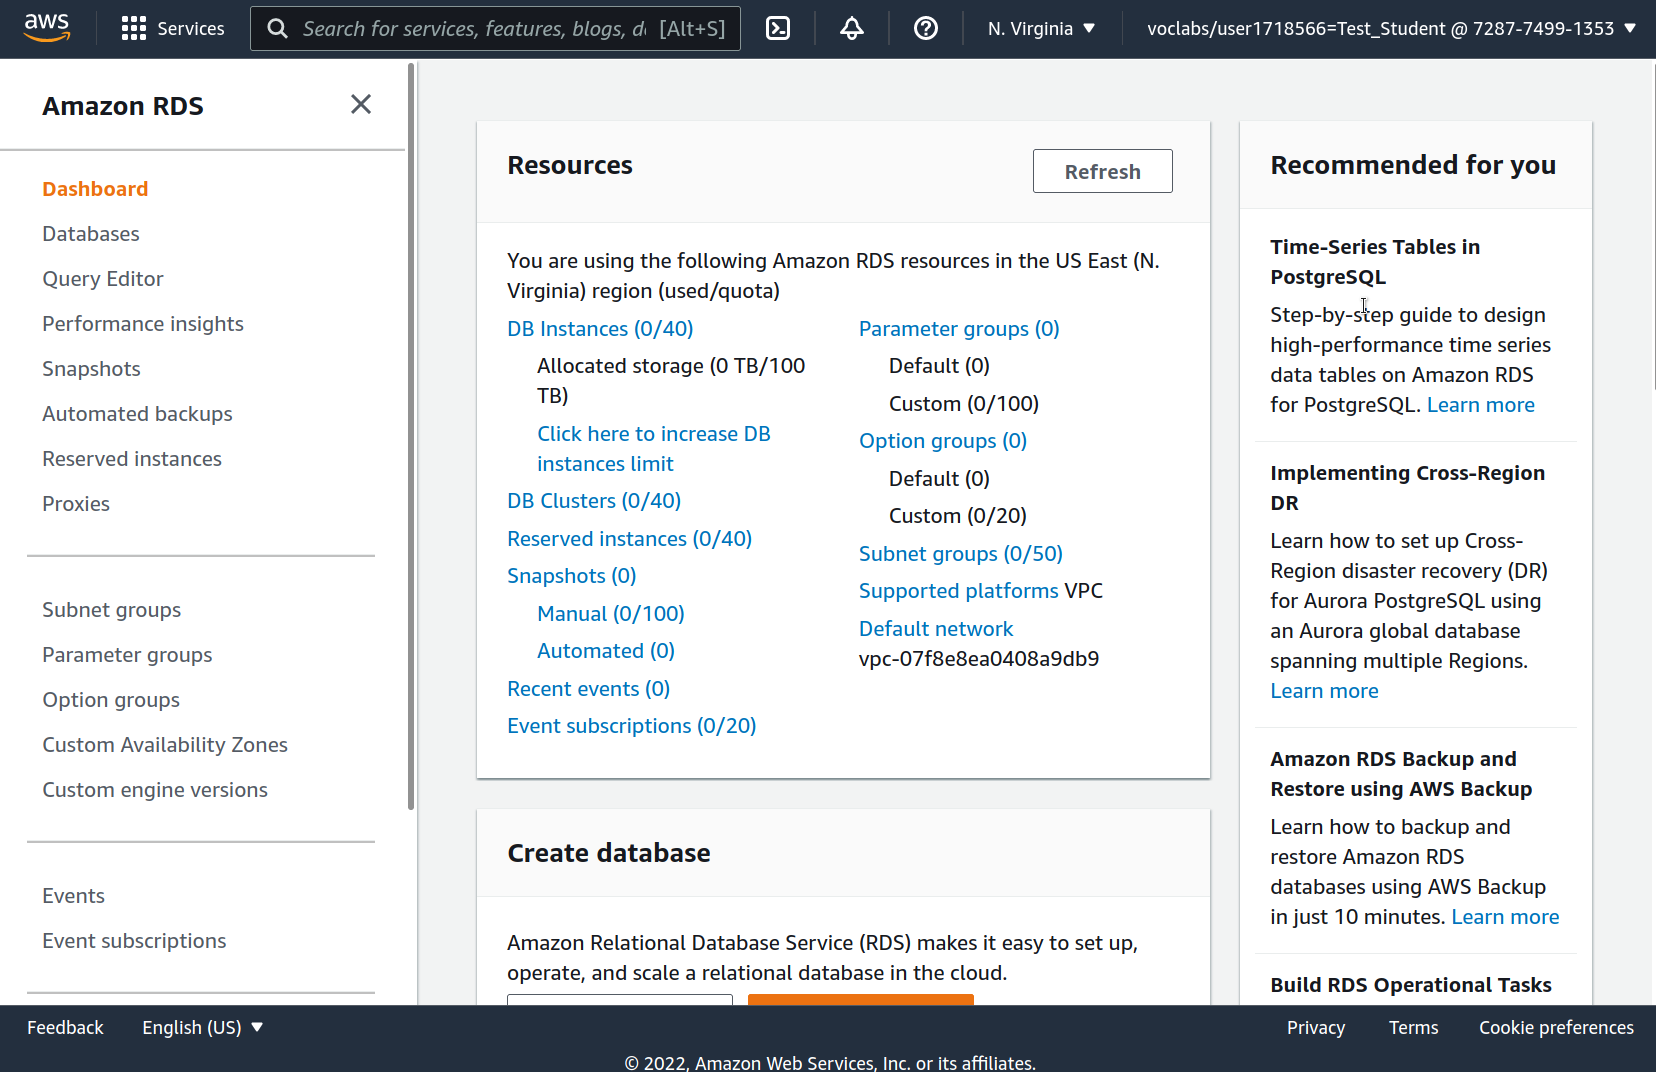
\includegraphics[width=\textwidth]{images/aws_2}
\end{figure}

This page should appear familar as it's very similar to the AWS EC2 instance page.
Let us create a new database by hitting the ``Create Database'' button.

\begin{figure}[H]
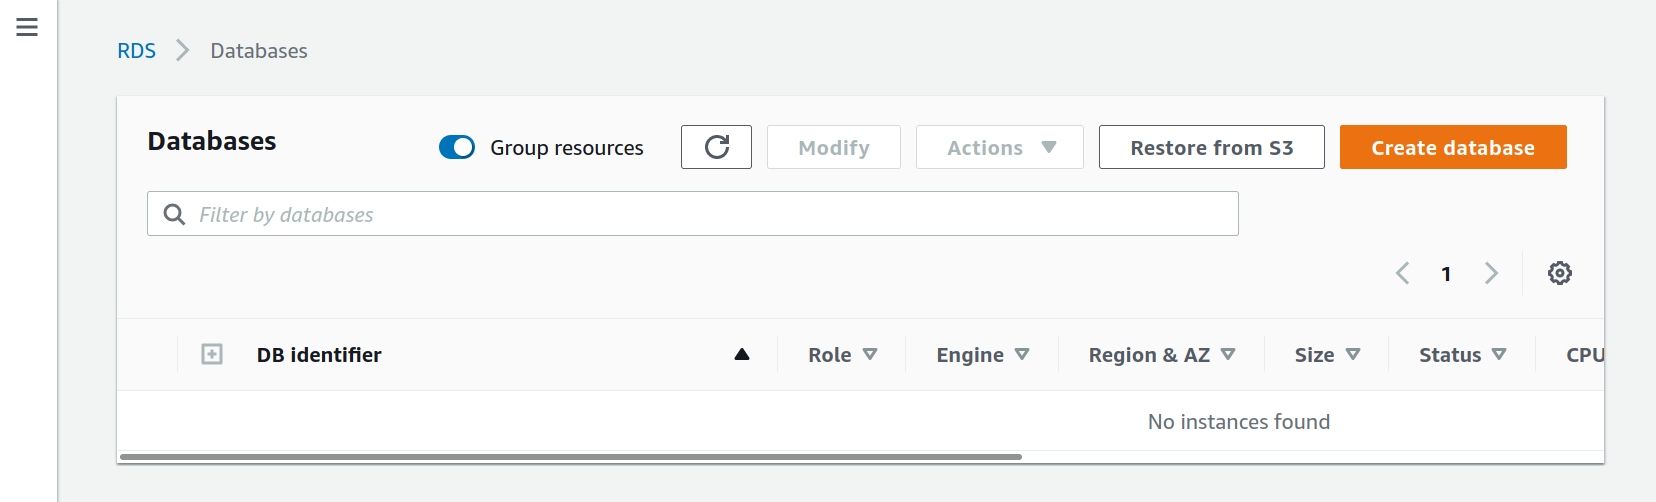
\includegraphics[width=\textwidth]{images/aws_3}
\end{figure}

\warning{
  In the next section we cannot use the Easy Create method as it tries to create a IAM account which is not allowed in the labs.
  Going forward we would typically do this using Terraform so we can easily avoid these restrictions.
}

\teacher{
  Feel free to talk about the other offerings here, but make sure to flame Oracle and Microsoft SQL Server.
  A good thing to point out is the Amazon Aurora which is the serverless version of RDS.
}

We will be creating a standard database so select standard and MySQL.
We will use version 8 to match the local version.

\begin{figure}[H]
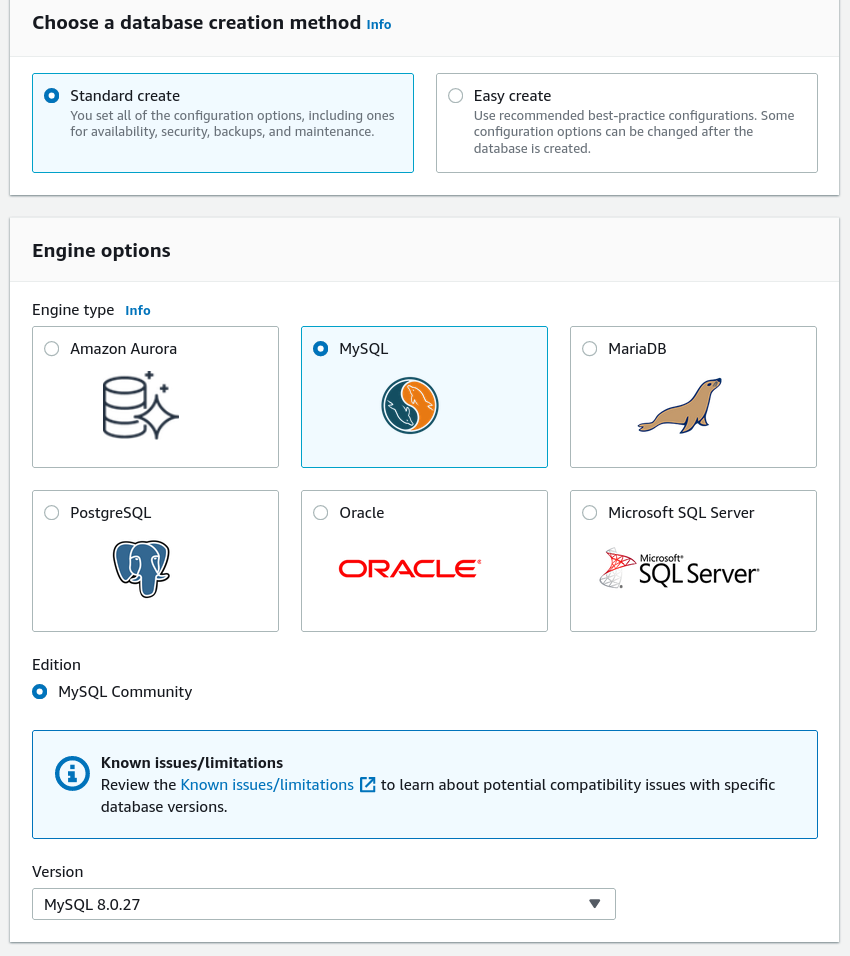
\includegraphics[width=\textwidth]{images/db1}
\end{figure}

For today we are going to use ``Free Tier'' but in the future,
you may wish to explore the different deployment options.
Please peruse the available different options.

\teacher{
  Walk through what Multi-AZ means aka Multiple Availability Zones.
}

\begin{figure}[H]
  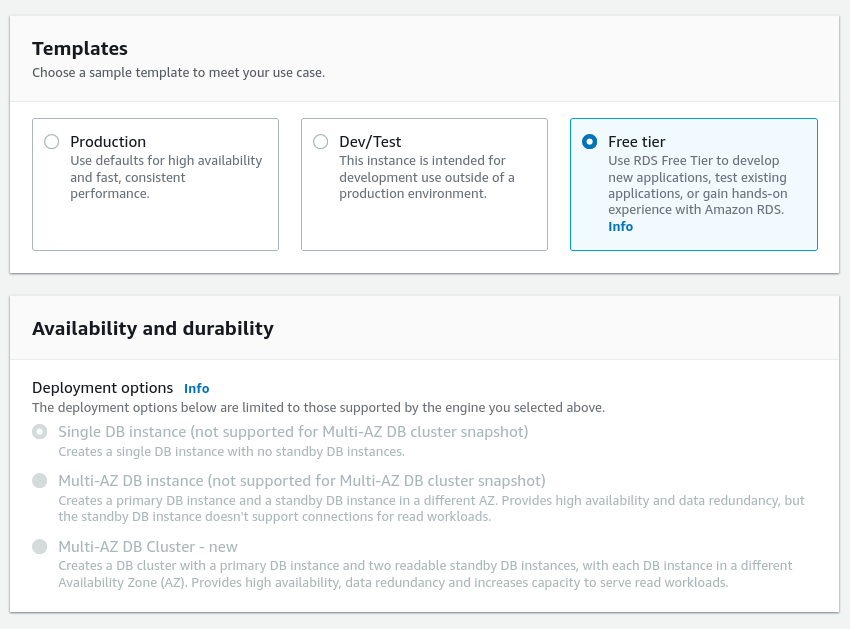
\includegraphics[width=\textwidth]{images/db2}
\end{figure}

Now we need to name our database and create credentials to connect via.
Please enter a reasonable password and keep this aside for later.
We will need it for our local docker-compose file.

\begin{figure}[H]
  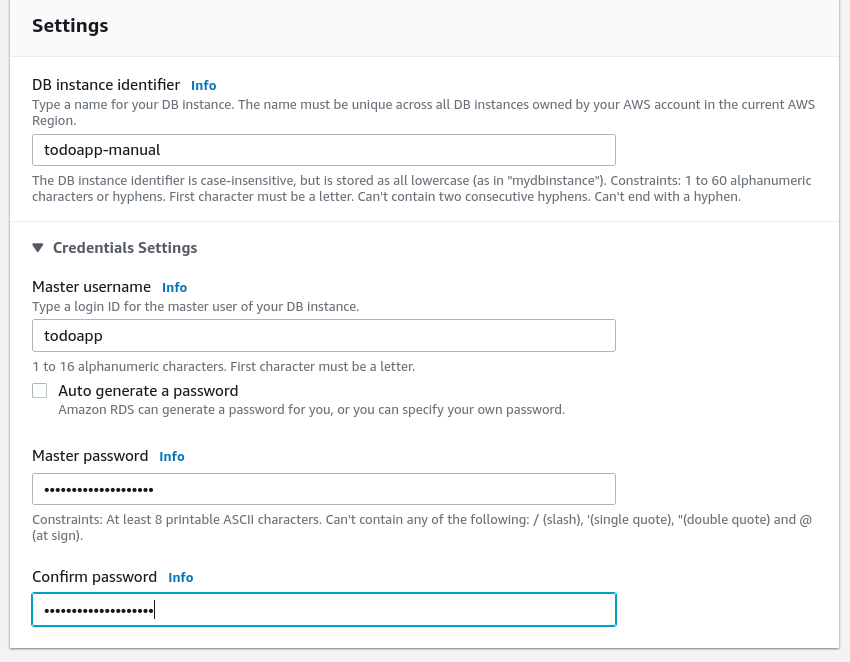
\includegraphics[width=\textwidth]{images/db3}
\end{figure}

We will use the default class type, t2.micro, which should be sufficient for this practical.

\teacher{
  May want to mention that burstable is not recommended for consistantly used databases.
  Usually DBs are memory focused and thus the standard or memory optimised are used.
}

\begin{figure}[H]
  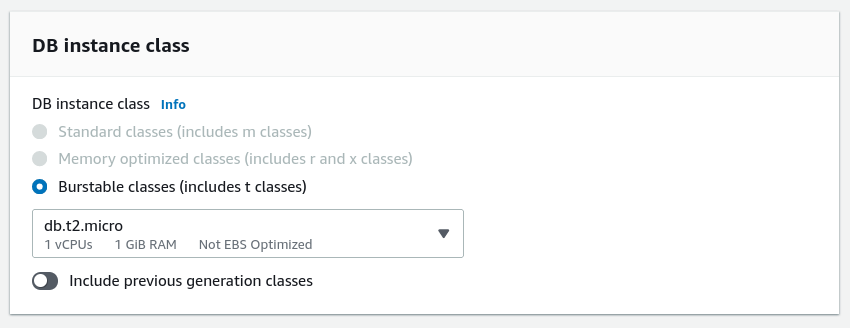
\includegraphics[width=\textwidth]{images/db4}
\end{figure}

For storage we will leave all the default options.

\begin{figure}[H]
  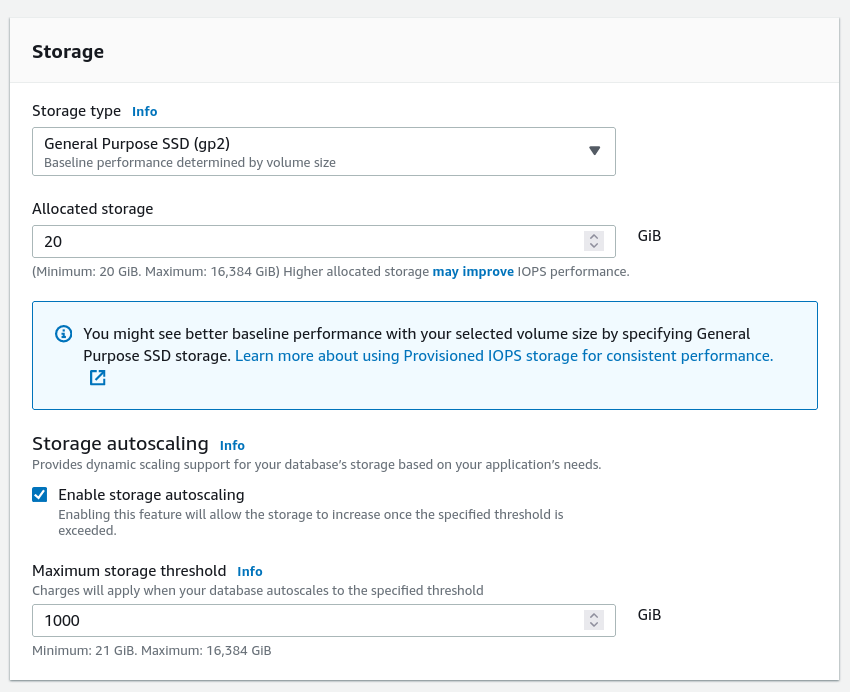
\includegraphics[width=\textwidth]{images/db5}
\end{figure}

In connectivity we need to make sure our instance is publicly available.
Usually you don't want to expose your databases publicly and, would instead, have a web server sitting in-front.
But for today we will be running that web server locally so for convenience we need public access.

When selecting public access as yes we have to create a new Security Group,
give this Security Group a sensible name.

\begin{figure}[H]
  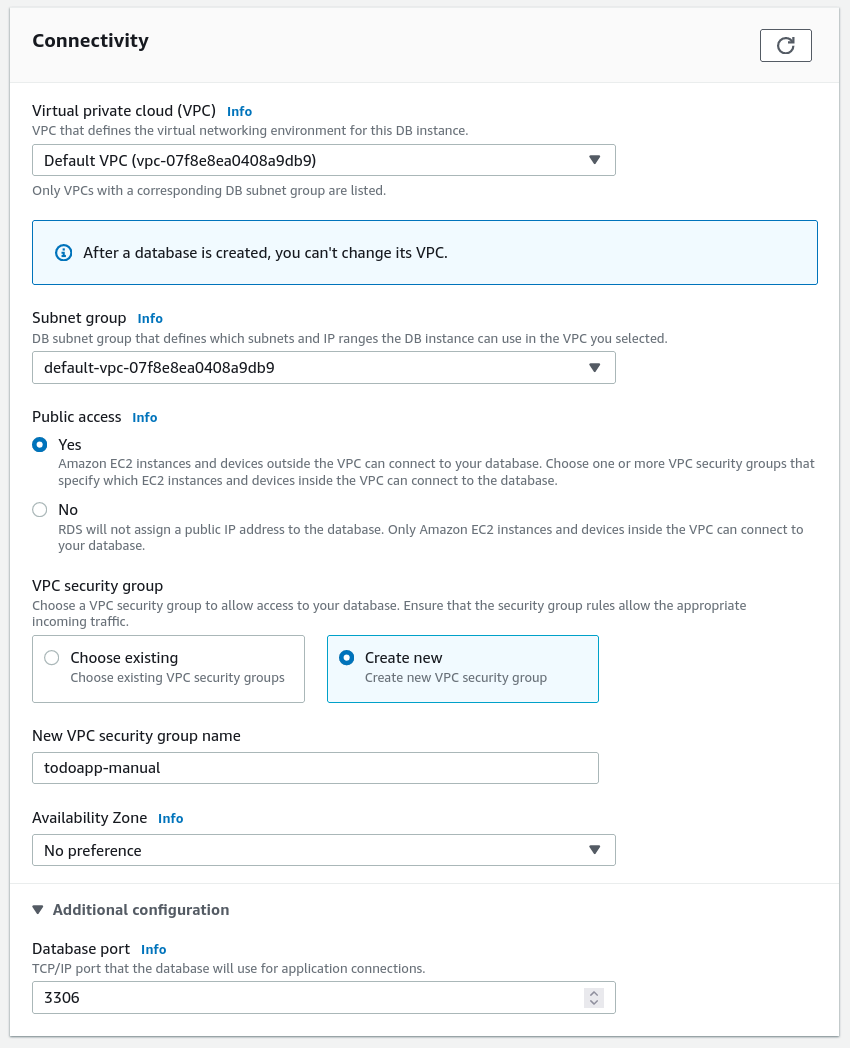
\includegraphics[width=\textwidth]{images/db6}
\end{figure}

We will leave the authentication as password based but we need to expand the ``Additional configuration''.
Fill in the ``Initial Database Name'' section to be ``todoapp'',
this is similar to what we had in the Docker Compose.

\teacher{
The other options here are to do with the parameters used to start the database,
it is uncommon to have to change these but this is where any settings you would pass in via cli to the db would be set.
}

\begin{figure}[H]
  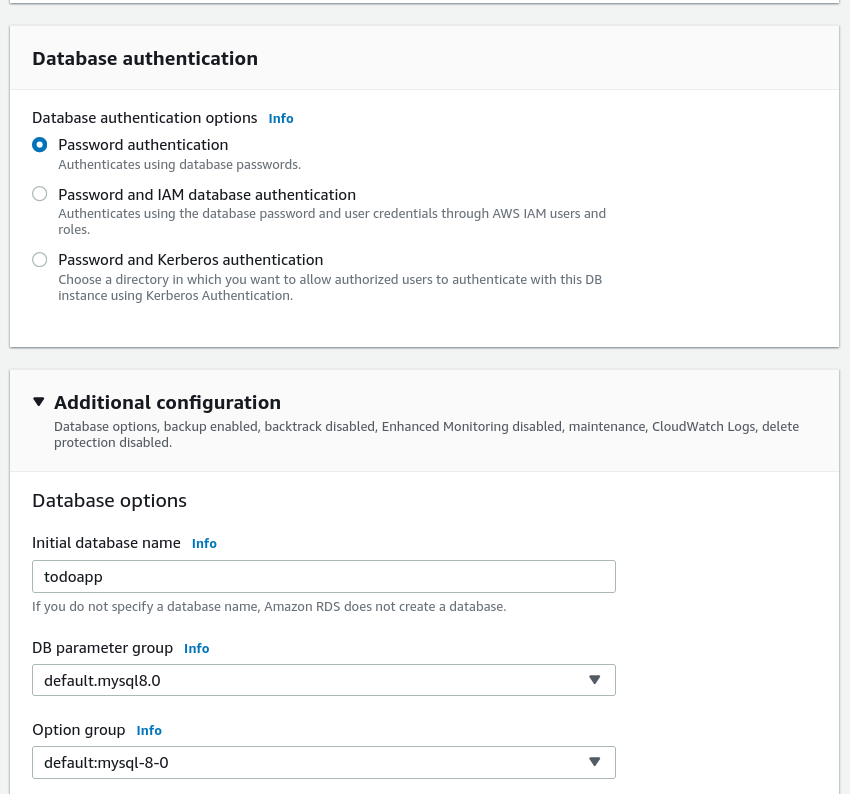
\includegraphics[width=\textwidth]{images/db7}
\end{figure}

Now we can click create which will take some time.

\begin{figure}[H]
  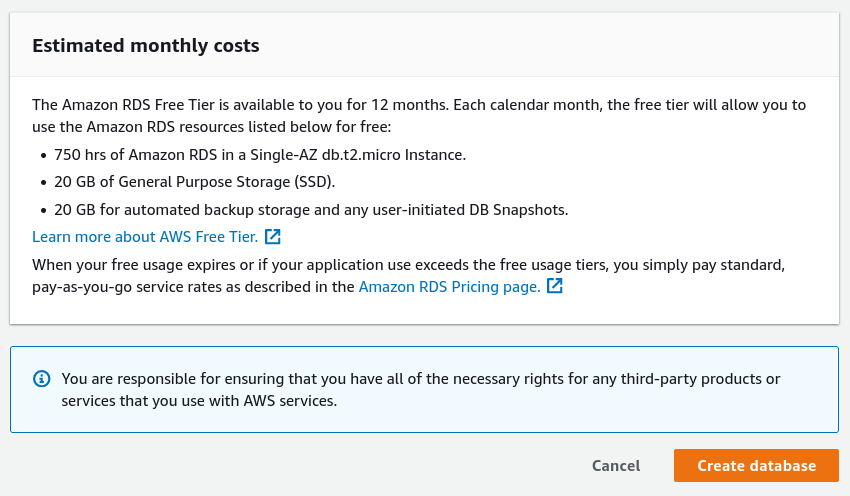
\includegraphics[width=\textwidth]{images/db8}
\end{figure}

Depending on your database it may take 10 to 30minutes to create,
the larger and more complicated the setup the longer it usually takes.
The database will also do a initial backup when its created.

\begin{figure}[H]
  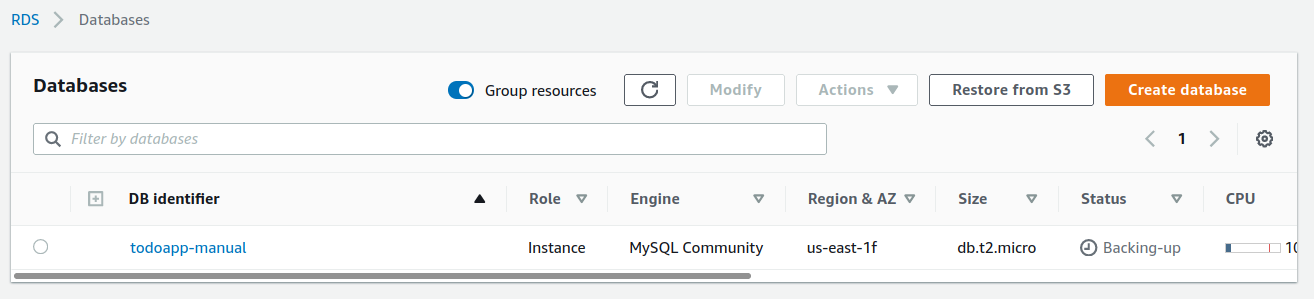
\includegraphics[width=\textwidth]{images/aws_4}
\end{figure}

When the database has finished being created you can select it to view the configuration and details.
In this menu we also see the endpoint address which we will need to copy into our docker compose file.

\begin{figure}[H]
  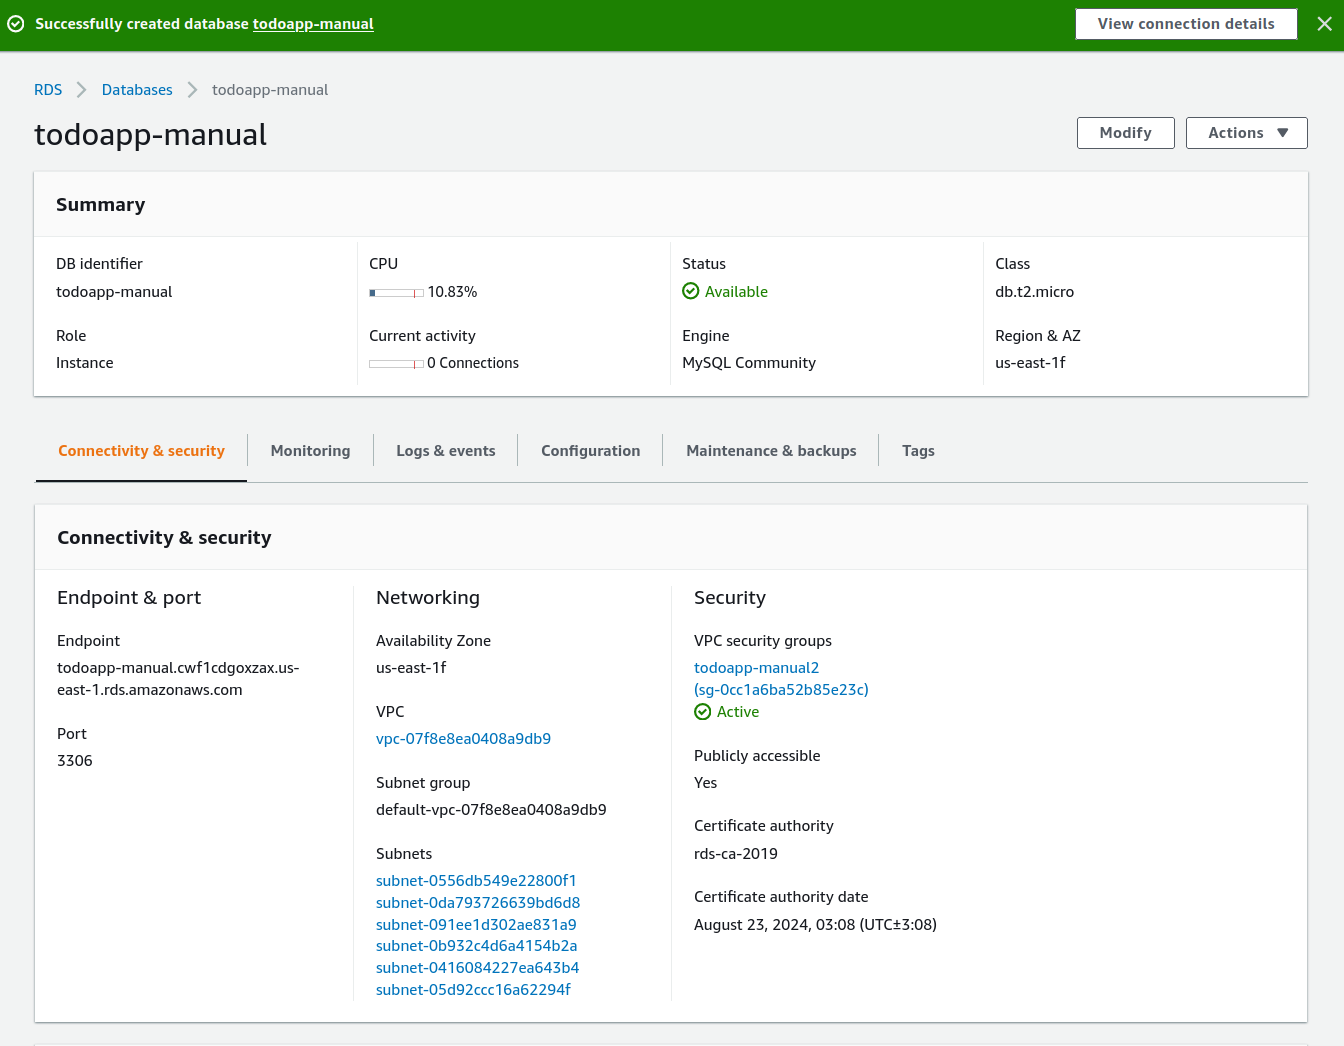
\includegraphics[width=\textwidth]{images/aws_5}
\end{figure}

So with the database all ready to go, let's get started on running our app.
First thing to do is to stop any running instances you have and then delete the database service from the docker compose.
Now we want to edit the \texttt{DB\_HOST} and \texttt{DB\_PASSWORD} to match what we set in AWS.
Below is an example of my configuration.

\begin{code}[language=docker-compose]{docker-compose.yml}
  version: '3.3'
  services:
    backend:
      image: ghcr.io/csse6400/todo-app:latest
      ports:
        - '8000:8000'
      environment:
        APP_ENV: 'local'
        APP_KEY: 'base64:8PQEPYGlTm1t3aqWmlAw/ZPwCiIFvdXDBjk3mhsom/A='
        APP_DEBUG: 'true'
        LOG_LEVEL: 'debug'
        DB_CONNECTION: 'mysql'
        DB_HOST: 'todoapp-manual.cwf1cdgoxzax.us-east-1.rds.amazonaws.com'
        DB_PORT: '3306'
        DB_DATABASE: 'todoapp'
        DB_USERNAME: 'todoapp'
        DB_PASSWORD: 'MyVerySecurePassword'
      command: sh -c "sleep 10 && php artisan migrate:refresh --seed && php artisan serve --host=0.0.0.0"
\end{code}

Now we can run \lstinline[]{$ docker-compose up}.
This will take a lot longer than before,
the reason behind this is that by default our lab is running in the US and it takes a lot longer to communicate to a DB half way across the world.

\begin{code}[language=shell,numbers=none]{}
  $ docker-compose up
  Creating network "remote_default" with the default driver
  Creating remote_backend_1 ... done
  Attaching to remote_backend_1
  backend_1  | Migration table not found.
  backend_1  | Migration table created successfully.
  backend_1  | Migrating: 2022_03_19_041557_create_todos_table
  backend_1  | Migrated:  2022_03_19_041557_create_todos_table (612.48ms)
  backend_1  | Seeding: Database\Seeders\TodoSeeder
  backend_1  | Seeded:  Database\Seeders\TodoSeeder (13,930.36ms)
  backend_1  | Database seeding completed successfully.
  backend_1  | Starting Laravel development server: http://0.0.0.0:8000
  backend_1  | [Mon Mar 21 04:45:34 2022] PHP 8.0.8 Development Server (http://0.0.0.0:8000) started
\end{code}

We can now also browse the app as before but with just a lot more lag.

\section{Deploying in AWS}\label{sect:terraform}

In this section we will deploy the application and database in AWS.
Rather than locally configuring a database as we did in the previous section,
we will deploy everything with Terraform.

\subsection{Authentication}

As we did last week,
specify the AWS provider we will use and download the Learner Lab credentials into a \texttt{credentials} file.
Once you have setup your \texttt{main.tf} and \texttt{credentials} files, run \lstinline{terraform init}.

\begin{code}[language=terraform]{main.tf}
terraform {
  required_providers {
    aws = {
      source = "hashicorp/aws"
      version = "~> 3.0"
    }
  }
}

provider "aws" {
  region = "us-east-1"
  shared_credentials_file = "./credentials"
}
\end{code}

\subsection{RDS Database}

Now would be a good time to browse the documentation for the RDS database in Terraform:
\url{https://registry.terraform.io/providers/hashicorp/aws/latest/docs/resources/db_instance}.
Using our manual configuration,
we can come up with a resource with the appropriate parameters as below:

\begin{code}[language=terraform]{main.tf}
locals {
  password = "foobarbaz" # this is bad
}

resource "aws_db_instance" "todoapp-database" {
  allocated_storage      = 20
  max_allocated_storage  = 1000
  engine                 = "mysql"
  engine_version         = "8.0.27"
  instance_class         = "db.t2.micro"
  name                   = "todoapp"
  username               = "todoapp"
  password               = local.password
  parameter_group_name   = "default.mysql8.0"
  skip_final_snapshot    = true
  vpc_security_group_ids = [aws_security_group.todoapp-database.id]
  publicly_accessible    = true

  tags = {
    Name = "todoapp-database"
  }
}
\end{code}

\noindent Remember to create an appropriate security group as we did through the user interface.

\begin{code}[language=terraform]{main.tf}
resource "aws_security_group" "todoapp-database" {
  name        = "todoapp-database"
  description = "Allow inbound MySQL traffic"

  ingress {
    from_port        = 3306
    to_port          = 3306
    protocol         = "tcp"
    cidr_blocks      = ["0.0.0.0/0"]
  }

  egress {
    from_port        = 0
    to_port          = 0
    protocol         = "-1"
    cidr_blocks      = ["0.0.0.0/0"]
    ipv6_cidr_blocks = ["::/0"]
  }

  tags = {
    Name = "todoapp-database"
  }
}
\end{code}

\subsection{Container on AWS}

As we mentioned in the Infrastructure as Code notes \cite{iac-notes},
in this course we will use Docker to configure machines and Terraform to configure infrastructure.
AWS has the ability to deploy Docker containers using a service known as Elastic Container Service (ECS).
Unfortunately, the AWS Learner Labs provided by AWS do not support ECS.

To resolve this issue,
we have created a Terraform module which allows us to deploy Docker images on EC2 instances and abstract over the underlying implementation.
The documentation and source for this Terraform module is available on Github: \url{https://github.com/CSSE6400/terraform/tree/main/container}.

Using the documentation of the module,
combined with the environment variables we know our backend requires based on the \texttt{docker-compose.yml} file,
we can develop a resource as below.

\begin{code}[language=terraform]{main.tf}
module "todoapp-backend" {
  source = "git::https://github.com/CSSE6400/terraform//container"
  
  image = "ghcr.io/csse6400/todo-app:latest"
  instance_type = "t2.micro"
  environment = {
    APP_ENV="local"
    APP_KEY="base64:8PQEPYGlTm1t3aqWmlAw/ZPwCiIFvdXDBjk3mhsom/A="
    APP_DEBUG="true"
    LOG_LEVEL="debug"
    DB_CONNECTION="mysql"
    DB_HOST=aws_db_instance.todoapp-database.address
    DB_PORT="3306"
    DB_DATABASE="todoapp"
    DB_USERNAME="todoapp"
    DB_PASSWORD=local.password
  }
  ports = {
    "80" = "8000"
  }
  security_groups = [aws_security_group.todoapp-backend.name]

  tags = {
    Name = "todoapp-backend"
  }
}
\end{code}

Note that we are passing the address of our remote database into the container as an environment variable.
This is a module which requires a source.
In our case, the source will be the Github repository created earlier.
Also notice that we map port 80 of the EC2 machine to port 8000 within the container,
we should create a security group to make the instance accessible.

\begin{code}[language=terraform]{main.tf}
resource "aws_security_group" "todoapp-backend" {
  name = "todoapp-backend"
  description = "Todo App HTTP and SSH access"

  ingress {
    from_port = 80
    to_port = 80
    protocol = "tcp"
    cidr_blocks = ["0.0.0.0/0"]
  }

  ingress {
    from_port = 22
    to_port = 22
    protocol = "tcp"
    cidr_blocks = ["0.0.0.0/0"]
  }

  egress {
    from_port = 0
    to_port = 0
    protocol = "-1"
    cidr_blocks = ["0.0.0.0/0"]
  }
}
\end{code}

You will also want to create an output block to expose the address of the instance.
  
\begin{code}[language=terraform]{main.tf}
output "url" {
  value = module.todoapp-backend.public_dns
}
\end{code}

This should give you a \texttt{main.tf} file which fully deploys a todo application.
If you haven't been applying as we go,
try and apply the Terraform file now.
If you have any issues,
ask your tutor for guidance.

\bibliographystyle{ieeetr}
\bibliography{books,ours}

\end{document}